%\newpage
%%%%%%%%%%%%%%%%%%%%%%%%%%%%%%%%%%%%%%%%%%%%%%%%%%%%%%%%%%%%%%%%%%%%%%%%%%%%%%%%
%%%%%%%%%%%%%%%%%%%%%%%%%%%%%%%%%%%%%%%%%%%%%%%%%%%%%%%%%%%%%%%%%%%%%%%%%%%%%%%%
\section{Princípios elementares no samba de gafieira}
\label{sec:principiosambagafieira}
\index{Princípios elementares!Samba de gafieira}

É evidente olhando aos profissionais da dança,
que cada pessoa tem uma forma particular de dançar, 
que carateriza e identifica a ela. Porém, 
dentro desse margem pessoal de trabalho, 
pode ser identificado quando uma pessoa está realizado um estilo de dança em particular,
por exemplo: samba de gafieira, forró, salsa, etc.
Assim, se conclui que existe um conjunto de caraterísticas na dança,
que provocam que estas sejam enquadradas num estilo particular;
estas caraterísticas não são todo ou nada, ou seja, 
não precisam cumprir-se todas para reconhecer um estilo de dança,
porém, quanto maior sejam as caraterísticas usadas mais fácil será enquadrar uma dança num estilo de dança em particular.

Os princípios elementares planteadas aqui, são uma tentativa de enumerar as caraterísticas,
que tenho observado, que provocam que um espectador ou dançarino,
veja ou perceba que se está dançando samba de gafieira.
\begin{description}
\item[Quadril avança, ombros e pé acompanham:]  Os movimentos, no samba de gafieira, 
que pretendem evocar uma estética relacionada com a malandragem,  geralmente iniciam no quadril;
isto provocará que as demais partes do corpo (pernas e torço) atuem a consequência para achar um novo equilíbrio.
Adicionalmente ajudará a que ao terminar o movimento, o peso de nosso corpo esteja imediatamente bem posicionado sobre um pé só.
Porém esta caraterística é só interessante, 
se o que o dançarino está procurando são elementos que contribuam a uma estética de malandragem;
para estéticas mais estilizadas, suaves e menos abruptas devemos estudar outros modos de transferência do peso do corpo.

%\item[Pisar com 100$\%$ do peso do corpo:] %quando se movimenta um pé.
\item[Transferência do peso do corpo:] %quando se movimenta um pé.
Uma característica comumente vista no samba de gafieira é uma estética que evoca à malandragem, 
uma forma de contribuir para obter esta estética é que ao movimentar um pé, 
este ao tocar o chão chegue com o 100\% do peso do corpo; realizar esta ação é fácil, 
se temos cumprido que nosso movimento inicie desde o quadril e não por esticar as pernas.

Assim, existe uma diferença com outros estilos de dança, 
como o bolero e o tango, 
onde se procura projetar uma estética de elegância e com movimentos fluidos;
nestes estilos, no movimento de pés, primeiro se aponta com a ponta do pé, sem levar o peso do corpo,
 e logo o peso é transferido ao lugar apontado, numa dinâmica continua de aponta e transfere o peso,
criando uma estética de elegância e fluides ao se deslocar.

Isto \textbf{não} quer dizer que a dinâmica de aponta e transfere seja menos interessante e não possa ser usada no samba de gafieira,
e sim que o dançarino deve escolher que imagem deseja projetar em cada momento:
malandragem, elegância ou misturas intermédias. 
Por este motivos, quando dançamos deve escolher cuidadosamente o jeito de transferir o peso do corpo. 

É interessante ressaltar que pode ser feito um paralelismo entre a música e o estudo da transferência de peso na dança;
no caso da música existem símbolos de \hyperref[sub:Articulation]{\textbf{articulação}} na notação musical, 
que indicam como as notas musicais devem ser executadas e articuladas entre sim;
por exemplo temos símbolos como: legato, staccato e tenuto;
que indicam que a articulação dos tons entre notas musicais consecutivas deve ser: fluida, ressaltada e  abrupta, respetivamente.
Pelo que se queremos ser coerentes com a música, 
ou com alguma porção dela que desejemos interpretar,
deveríamos escolher cuidadosamente nosso modo de transferência de peso,
para fazê-lo fluido, ressaltado, abrupto, etc.


\item[Ter um bom abraço no samba de gafieira:] Como já foi mencionado na Seção \ref{sec:PrincipioGeral}, 
ter uma boa conexão na dança é muito importante para uma boa transferência de informação na condução; 
porém, existem particularidades desta conexão no samba de gafieira que devem ser ressaltadas.

Por exemplo, na maioria de movimentos se usa o \hyperref[def:abracodedanca]{\textbf{abraço de dança}};
mas, particularmente no samba de gafieira, se precisa que o braço esquerdo da dama tenha contato
e rodeie, pela parte externa, ao braço direito do condutor; 
de modo  que o seguidor não se debruce sobre o condutor,
e sim que mantenha um atrito entre os braços.
A importância deste contato radica em que o condutor em algumas situações precisa transmitir instruções 
que provoquem uma ``sacada de perna'' do seguidor (ex: Edmundo, sacadas, etc.), 
e isto é transmitido quando o condutor realiza um movimento de rotação do tórax no plano axial.  
Rotando em sentido horário para tirar a perna direita do seguidor, 
e em sentido anti-horário para tirar a perna esquerda.
É neste ponto que esse atrito entre os braços é importante, 
pois quando se realiza o movimento de rotação anti-horário, se não existisse o atrito,
o tórax do condutor giraria no vácuo, sem afetar o tórax do seguidor ou afetando muito pouco;
assim, o atrito garante que esta informação na torção chegue com maior eficacia ao seguidor,
ver Figura \ref{fig:torcao-abraco}.
\begin{figure}[h]
  \centering
    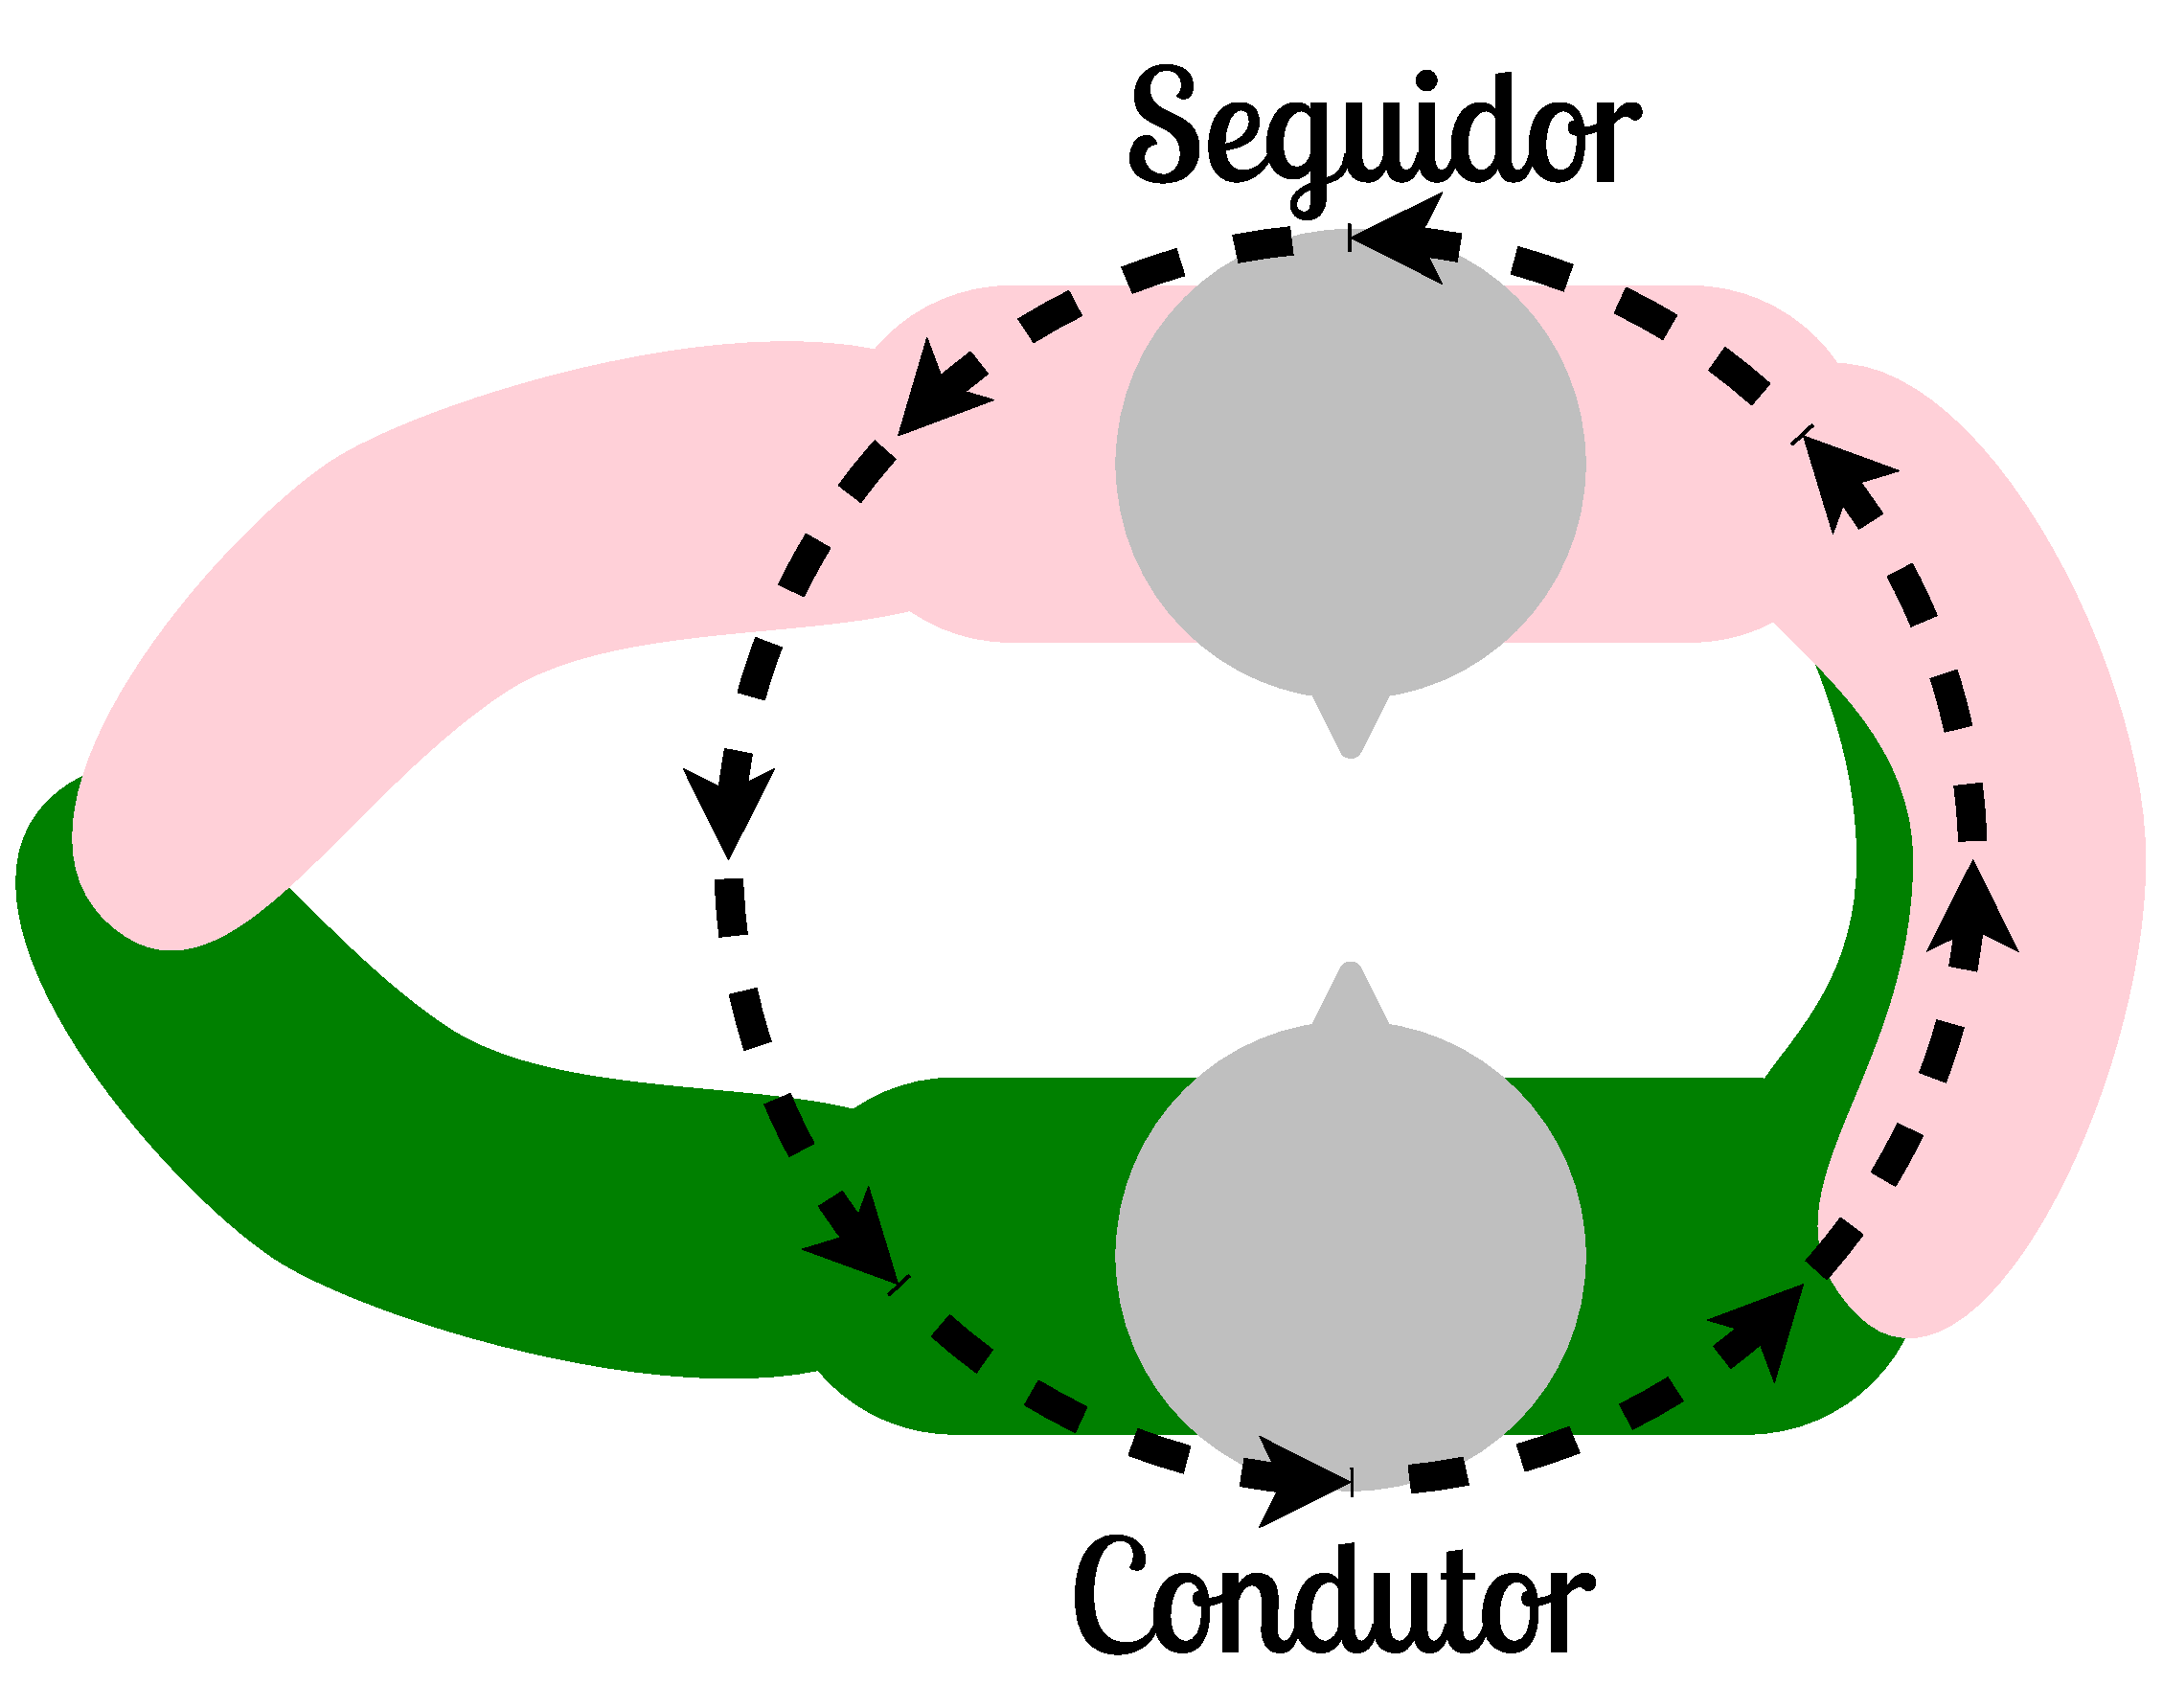
\includegraphics[width=0.43\textwidth]{chapters/cap-normas/torcao-abraco.eps}
\caption{Transferência de informação de condução ao seguidor, mediante do torção do tórax no sentido anti-horário.}
\label{fig:torcao-abraco}
\end{figure}

Por outro lado, em alguns momentos na dança, no samba de gafieira, usaremos um abraço de dança mais separado,
para realizar passos como o ``picadilho''; em estas circunstancias, é o braço direito do seguidor,
que precisa em todo momento estar \hyperref[def:brazosfirmes]{\textbf{firme}}, 
mantendo uma ativação muscular e diminuição dos graus de liberdade,
para que toda a informação enviada pelo condutor atravesse os braços e o tórax do seguidor,
e chegue sem degradação até o quadril, onde se provocará a movimentação de pés planejado pelo condutor.

\item[Abraço uniforme do condutor:] Continuando com as particularidades do abraço,
mas agora no âmbito da distancia de separação entre o \hyperref[def:Par]{\textbf{par}} durante o tempo que dure o abraço num movimento.
É importante ressaltar que deve-se manter uma regularidade na distancia de separação
e evitar um ``abraço sanfona'' durante um movimento, ou seja um abraço onde o condutor, num mesmo movimento, as vezes 
aperta demais ao seguidor e outras vezes deixe ele solto e mais separado.
É claro que na dança existe esta irregularidade do abraço para cada movimento; 
mas, esta característica é uma coisa consciente e projetada 
pelo condutor em função da técnica necessária para realizar um movimento; 
e em nenhum caso deve ser uma coisa fora de controle.

Um momento onde é altamente importante esta regularidade, 
é durante passos como o ``gancho redondo''.
Por outro lado, temos momentos em que precisaremos ajustar a distancia do abraço,
antes do inicio do passo, para mais perto no caso do ``pião'' e para mais longe no caso do ``picadilho''.

\item[Procurar o paralelismo de ombros no par:] 
Um ponto muito cobrado, na dança de salão é manter a linha de visão no \hyperref[def:Par]{\textbf{par}},
em samba de gafieira esta caraterística é obtida mantendo sempre paralelas as linhas dos ombros no par.
Isto além de um ganho estético tem interessantes caraterísticas técnicas;
pois se a combinamos com a ideia de manter sempre a mesma distancia no par;
chegamos a um ponto onde poderemos estabelecer uma condução por indução, ou condução sem contato.

A responsabilidade de manter este paralelismo de ombros é do \hyperref[def:Seguidor]{\textbf{seguidor}},
pois este deve ``seguir'' o movimento do \hyperref[def:Condutor]{\textbf{condutor}}.
Por outro lado o condutor tem a responsabilidade de realizar os movimentos com uma velocidade e clareza necessárias, 
para que estes possam ser acompanhados pelo seguidor.

\item[Conduzir pelo tórax não pelos braços:] 
Se conseguimos ter paralelismo na linha dos ombros,
e se procuramos manter sempre a mesma distancia, 
e linha de visão com o \hyperref[def:Par]{\textbf{par}}, 
sem a necessidade do uso dos braços;
pode-se deduzir que, nestas dinâmicas corporais,
é o tórax do \hyperref[def:Condutor]{\textbf{condutor}} quem guia ao \hyperref[def:Seguidor]{\textbf{seguidor}}.
Isto implica que os braços tem o papel de brindar sustento para a transferência de informação da condução,
porém os braços do condutor, não são os executantes e protagonistas da condução;
sendo, principalmente o tórax do condutor, a fonte mecânica desta informação.
Este dado é muito relevante em passos como o ``Romário'' ou o ``gancho redondo'',
onde é o tórax, e não os braços, do condutor que leva ao seguidor de um lado a outro. 

\item[O pé de apoio deve apontar ao par:] 
Quando nos encontremos numa postura, em que o peso do corpo está definido totalmente num pé;  
ou seja, quando não estamos num movimento de transferência de peso;
o pé que contem o peso do corpo debe apontar a um ponto médio entre os pés do \hyperref[def:Par]{\textbf{par}} de dança.
Esta caraterística tem um proposito técnico além de estético;
dado que o corpo tende a ir em direção a onde está apontando nosso pé;
assim, ao apontar sempre ao par, 
garantimos que em todo momento procuraremos a proximidade e teremos uma linha de visão  com ele.
Uma boa metáfora, é pensar que a ponta de nosso pé é uma bússola que aponta ao norte, que é nosso par.
\end{description}
